
%(BEGIN_QUESTION)
% Copyright 2009, Tony R. Kuphaldt, released under the Creative Commons Attribution License (v 1.0)
% This means you may do almost anything with this work of mine, so long as you give me proper credit

The sensitivity and linearity of a pneumatic force-balance instrument may be improved with the addition of a {\it pneumatic amplifying relay} to amplify the response of the flapper/nozzle assembly.  It other words, the inclusion of an amplifier into the system increases the system's {\it gain}.  Explain what happens, step by step, in the system shown, if force is applied to the lever by someone's thumb:

$$\includegraphics[width=15.5cm]{i00201x01.eps}$$

\vskip 10pt

Also, determine whether the mechanism will still produce the same amount of output pressure for any given amount of applied force without the amplifying relay in place.  In other words, if we removed the relay from the system, would the output pressure be greater than before, less than before, or the same as before given the same force applied to the lever?

$$\includegraphics[width=15.5cm]{i00201x05.eps}$$

\vskip 10pt

Challenge question: if we reduced the restriction (orifice) bore size in this system such that less air flowed through the nozzle, would the output pressure be greater than before, less than before, or the same as before given the same force applied to the lever?

\underbar{file i00201}
%(END_QUESTION)





%(BEGIN_ANSWER)

The particular pneumatic amplifying relay shown is the one typically used in Foxboro pneumatic instruments.  It is not the only type of amplifying relay design, but a very common one.

$$\includegraphics[width=15.5cm]{i00201x02.eps}$$

If the lever is pushed toward the nozzle by an external force, the following will happen:

\medskip
{\item{} Pressure upstream of the nozzle will increase, as the nozzle becomes more restricted by the flapper.
{\item{} This pressure, going to the relay through the ``input'' port, will push {\it up} on the relay diaphragm.
{\item{} The relay diaphragm lifts up, pushing the stem valve closer to its seat, and lifting the ball off of its seat.
{\item{} As the ball lifts off its seat, more supply air is allowed to go into the area between the ball and stem.
{\item{} As the stem closes on its seat, the passage from this middle area to the vent port becomes more restrictive.
{\item{} As a result of the previous two factors, the output air pressure to the bellows will increase dramatically.
{\item{} The bellows will expand, pushing to the right on the lever.
{\item{} As the flapper will move to the right until a condition of equilibrium is reached with the force from the thumb.
\medskip

The operation of the pneumatic relay might require a bit more explanation for full understanding.  The ``input'' pressure sent to the relay from the nozzle tube pushes against the full area of the diaphragm, creating an upward force.  Since the area above the diaphragm is vented (at atmospheric pressure), there can be no substantial pressure buildup on the top side of the diaphragm, and thus no downward force generated by the diaphragm to counter the input pressure's upward force:

$$\includegraphics[width=15.5cm]{i00201x03.eps}$$

This force acts to lift the ``ball'' valve off its seat and also close the cone-shaped ``stem valve,'' adding more pressure to the output chamber by opening the passage for supply air to enter and closing the passage for air to vent, respectively:

$$\includegraphics[width=15.5cm]{i00201x04.eps}$$

The only force opposing the diaphragm's upward motion is a small leaf spring pressing down against the ball.  This spring is not very strong, meaning that small changes in input pressure result in large changes in output pressure.  In other words, the pneumatic amplifying relay has a very large {\it gain}.

Pneumatic relays such as this serve the same purpose as operational amplifiers in electronic circuits: amplifiers with extremely high gains, used within negative feedback loops to achieve some lesser amount of amplification that is very nearly linear.  In this particular example, the final result (flapper, nozzle, lever, relay, and bellows) is a force-balance system that aggressively responds to any external force applied to the lever, such as the force exerted by someone's thumb.  In a real pneumatic instrument, this external force would represent some signal or process variable, and the balancing pressure at the bellows would be the instrument's pneumatic output signal.

\vskip 10pt

The presence or absence of the pneumatic amplifying relay does {\it not} alter the pressure/force relationship of this mechanism.  The relay merely increases sensitivity to small changes in force, and increases the speed of response.

\vskip 10pt

Answer to challenge question: although narrowing the restriction would decrease nozzle air flow, this would have no effect on the pressure/force relationship of this mechanism.  It is {\it still} a force-balance system where bellows force must equal applied force to reach a state of equilibrium, and this bellows force is strictly a function of nozzle pressure ($F = PA$) not nozzle flow rate.

\vskip 10pt

It should be noted that the actual gain of the pneumatic amplifier ($\Delta P_{out} \over \Delta P_{in}$) is irrelevant, so long as it is arbitrarily large.  This is analogous to the open-loop voltage gain of an operational amplifier being largely irrelevant to the overall voltage gain of a negative-feedback circuit.  In other words, the presence of this amplifying relay does not alter the input force / output pressure relationship of this pneumatic mechanism.

\vskip 10pt

In order to alter the pressure/force relationship of this mechanism, one would have to alter the feedback components: either change the effective area of the bellows, or the moment arm through which it acts to counteract the applied force.


%(END_ANSWER)





%(BEGIN_NOTES)


%INDEX% Basics, pneumatics: force-balance mechanism

%(END_NOTES)


